% ============================================================
%  يُترجَم بـ XeLaTeX  (في Overleaf: Menu → Compiler → XeLaTeX)
%  الخط: Amiri (متوفر في Overleaf، أو حمّله من github.com/aliftype/amiri)
% ============================================================
\documentclass[12pt,a4paper]{article}
\usepackage[a4paper,margin=1.7cm,top=2.3cm,bottom=2.9cm,headheight=15pt,footskip=1.5cm]{geometry}
\usepackage{amsmath,amssymb}
\usepackage{icomma}
\usepackage[english,bidi=default,layout=lists]{babel}
\babelprovide[import,main]{arabic}
\babelfont{rm}[Scale=1.08]{Amiri}
\babelfont{sf}[Scale=1.08]{Amiri}
\usepackage[most]{tcolorbox}
\usepackage{tikz}
\usetikzlibrary{arrows.meta,calc,shadings}
\usepackage{array}
\usepackage{colortbl}
\usepackage{fancyhdr}
\usepackage{titlesec}
\usepackage{enumitem}
\usepackage{collcell}
\usepackage{needspace}
\usepackage{etoolbox}
\newcolumntype{C}{>{\collectcell\ar}c<{\endcollectcell}}
\pretocmd{\section}{\Needspace{15\baselineskip}}{}{}
\pretocmd{\subsection}{\Needspace{11\baselineskip}}{}{}

\definecolor{cDef}{HTML}{1F4E9C}
\definecolor{cThm}{HTML}{B3261E}
\definecolor{cRem}{HTML}{2E7D32}
\definecolor{cEx}{HTML}{C76B00}
\definecolor{cMeth}{HTML}{6A1B9A}
\definecolor{cSol}{HTML}{00695C}
\definecolor{cSec}{HTML}{1F3A68}

\titleformat{\section}{\Large\bfseries\color{cSec}}{\thesection.}{0.6em}{}[{\color{cSec!60}\titlerule[1pt]}]
\titleformat{\subsection}{\large\bfseries\color{cThm!85!black}}{\thesubsection.}{0.5em}{}
\titlespacing*{\section}{0pt}{14pt}{8pt}
\titlespacing*{\subsection}{0pt}{10pt}{5pt}
\setlength{\parindent}{0pt}
\setlength{\parskip}{4pt}
\setlist{itemsep=2pt,topsep=3pt}

\newtcolorbox{arbox}[3][]{enhanced,
  colback=#2!5,colframe=#2!80!black,arc=2mm,boxrule=0.8pt,
  left=6pt,right=6pt,top=8pt,bottom=5pt,
  fonttitle=\bfseries,coltitle=white,
  title={\foreignlanguage{arabic}{#3}},
  attach boxed title to top right={xshift=-5mm,yshift=-3mm},
  boxed title style={colback=#2!80!black,arc=1.5mm,boxrule=0pt},
  before upper={\selectlanguage{arabic}},
  before skip=8pt,after skip=8pt,breakable,#1}
\newenvironment{BOX}[2]{\begin{otherlanguage}{english}\begin{arbox}{#1}{#2}}{\end{arbox}\end{otherlanguage}}
\newenvironment{tarif}[1][تعريف]{\begin{BOX}{cDef}{#1}}{\end{BOX}}
\newenvironment{khassia}[1][خاصية]{\begin{BOX}{cThm}{#1}}{\end{BOX}}
\newenvironment{molahada}[1][ملاحظة]{\begin{BOX}{cRem}{#1}}{\end{BOX}}
\newenvironment{mithal}[1][مثال]{\begin{BOX}{cEx}{#1}}{\end{BOX}}
\newenvironment{tariqa}[1][طريقة]{\begin{BOX}{cMeth}{#1}}{\end{BOX}}

\newcounter{exo}
\newenvironment{tamrin}[1]{\stepcounter{exo}\begin{BOX}{cSec}{التمرين \theexo: #1}}{\end{BOX}}
\newenvironment{hal}{\Needspace{12\baselineskip}\begin{otherlanguage}{english}\begin{arbox}[breakable]{cSol}{حل التمرين \theexo}}{\end{arbox}\end{otherlanguage}}

\newenvironment{LTR}{\begin{otherlanguage}{english}}{\end{otherlanguage}}
\newcommand{\ar}[1]{\foreignlanguage{arabic}{#1}}

\renewcommand{\dots}{\mathinner{\ldotp\ldotp\ldotp}}
\renewcommand{\ldots}{\mathinner{\ldotp\ldotp\ldotp}}
\renewcommand{\cdots}{\mathinner{\cdotp\cdotp\cdotp}}
\newcommand{\N}{\mathbb{N}}
\newcommand{\Z}{\mathbb{Z}}
\newcommand{\D}{\mathbb{D}}
\newcommand{\Q}{\mathbb{Q}}
\newcommand{\R}{\mathbb{R}}
\newcommand{\pgcd}{\operatorname{PGCD}}
\newcommand{\ppcm}{\operatorname{PPCM}}

% \NLseg{a}{b}{[}{]} ; \NLright{a}{[} ; \NLleft{b}{]}  (interval on a number line)
\newcommand{\NLseg}[4]{\begin{LTR}\begin{tikzpicture}[baseline=-0.6ex]
 \draw[-{Stealth[length=2mm]},gray!70](0,0)--(3.4,0);
 \draw[line width=2pt,cThm!80!black](0.7,0)--(2.7,0);
 \node[cThm!80!black,font=\LARGE] at (0.7,0){$#3$};
 \node[cThm!80!black,font=\LARGE] at (2.7,0){$#4$};
 \node[below=3pt,font=\footnotesize] at (0.7,0){$#1$};
 \node[below=3pt,font=\footnotesize] at (2.7,0){$#2$};
\end{tikzpicture}\end{LTR}}
\newcommand{\NLright}[2]{\begin{LTR}\begin{tikzpicture}[baseline=-0.6ex]
 \draw[-{Stealth[length=2mm]},gray!70](0,0)--(3.4,0);
 \draw[line width=2pt,cThm!80!black](1.3,0)--(3.3,0);
 \node[cThm!80!black,font=\LARGE] at (1.3,0){$#2$};
 \node[below=3pt,font=\footnotesize] at (1.3,0){$#1$};
\end{tikzpicture}\end{LTR}}
\newcommand{\NLleft}[2]{\begin{LTR}\begin{tikzpicture}[baseline=-0.6ex]
 \draw[-{Stealth[length=2mm]},gray!70](0,0)--(3.4,0);
 \draw[line width=2pt,cThm!80!black](0.05,0)--(2.1,0);
 \node[cThm!80!black,font=\LARGE] at (2.1,0){$#2$};
 \node[below=3pt,font=\footnotesize] at (2.1,0){$#1$};
\end{tikzpicture}\end{LTR}}

% ---------- social-media icons (pure TikZ) ----------
\definecolor{cFB}{HTML}{1877F2}
\definecolor{cTG}{HTML}{229ED9}
\definecolor{cIG1}{HTML}{FEDA75}
\definecolor{cIG2}{HTML}{D62976}
\definecolor{cIG3}{HTML}{4F5BD5}
\newcommand{\fbicon}{\begin{LTR}\begin{tikzpicture}[baseline=-0.75ex,x=1em,y=1em]
 \fill[cFB] (0,0) circle (0.55);
 \node[white,inner sep=0,font=\usefont{TU}{lmss}{bx}{n}\small] at (0.04,-0.02) {f};
\end{tikzpicture}\end{LTR}}
\newcommand{\igicon}{\begin{LTR}
\begin{tikzpicture}[baseline=-0.75ex,x=1em,y=1em]
 \shade[lower left=cIG1,lower right=cIG2,upper left=cIG2,upper right=cIG3,rounded corners=0.28em] (-0.55,-0.55) rectangle (0.55,0.55);
 \draw[white,line width=0.09em,rounded corners=0.18em] (-0.36,-0.36) rectangle (0.36,0.36);
 \draw[white,line width=0.09em] (0,0) circle (0.17);
 \fill[white] (0.22,0.22) circle (0.05);
\end{tikzpicture}\end{LTR}}
\newcommand{\tgicon}{\begin{LTR}
\begin{tikzpicture}[baseline=-0.75ex,x=1em,y=1em]
 \fill[cTG] (0,0) circle (0.55);
 \fill[white] (-0.33,0.0) -- (0.32,0.27) -- (0.2,-0.3) -- (0.0,-0.15) -- (-0.08,-0.28) -- (-0.08,-0.08) -- cycle;
 \fill[cTG!70!black] (-0.08,-0.08) -- (0.25,0.2) -- (0.0,-0.15) -- (-0.08,-0.28) -- cycle;
\end{tikzpicture}\end{LTR}}
% page number: black box, white two-digit number, at the right of the social row
\newcommand{\PageBox}{\begin{LTR}\tikz[baseline=(p.base)]\node[fill=black,text=white,inner sep=2.5pt,minimum width=1.6em,minimum height=1.3em,font=\usefont{TU}{lmss}{bx}{n}\small](p){\ifnum\value{page}<10 0\fi\arabic{page}};\end{LTR}}
% visual left-to-right order: Telegram | Instagram | Facebook | page box
\newcommand{\SocialRow}{\begin{otherlanguage}{english}%
 \ar{\textbf{الأستاذ سوايسية هشام للرياضيات}}\ \tgicon\hfill
 \textbf{prof\_hicham\_math}\ \igicon\hfill
 \ar{\textbf{الأستاذ سوايسية هشام للرياضيات}}\ \fbicon\hspace{2.2em}\PageBox\end{otherlanguage}}

\pagestyle{fancy}
\fancyhf{}
\renewcommand{\headrulewidth}{0.6pt}
\renewcommand{\footrulewidth}{0.4pt}
% \SetHeader{right head: document title}{left head: level -- stream}
\newcommand{\SetHeader}[2]{%
 \fancyhead[C]{\parbox{\textwidth}{\ar{#1\hfill #2}}}%
 \fancyfoot[C]{\parbox{\textwidth}{\small\SocialRow}}}
\usepackage{tkz-tab}
\usepackage{multicol}
% variation / sign table (LTR)
\newenvironment{TAB}{\par\begin{center}\begin{LTR}\begin{tikzpicture}[scale=0.95,every node/.style={font=\small}]}{\end{tikzpicture}\end{LTR}\end{center}}
% grid + axes, clipped: \begin{GR}{xmin}{xmax}{ymin}{ymax}{unit cm}
\newenvironment{GR}[5]{\par\begin{center}\begin{LTR}\begin{tikzpicture}[x=#5cm,y=#5cm,font=\footnotesize]
 \draw[gray!25,very thin] (#1,#3) grid (#2,#4);
 \draw[-{Stealth[length=2mm]}] (#1,0)--(#2+0.3,0) node[below left]{$x$};
 \draw[-{Stealth[length=2mm]}] (0,#3)--(0,#4+0.3) node[below left]{$y$};
 \node[below left] at (0,0){$O$};
 \begin{scope}\clip (#1,#3) rectangle (#2,#4);}
{\end{scope}\end{tikzpicture}\end{LTR}\end{center}}
\newcommand{\Ticks}[2]{\foreach \t in {#1} \node[below,font=\scriptsize] at (\t,0){$\t$}; \foreach \t in {#2} \node[left,font=\scriptsize] at (0,\t){$\t$};}
\newcommand{\bx}[1]{\ensuremath{\colorbox{cDef!12}{$\displaystyle #1$}}}
\newcommand{\TwoCol}[4]{\par\begin{LTR}\noindent\begin{minipage}[t]{#1\textwidth}\selectlanguage{arabic}#2\end{minipage}\hfill\begin{minipage}[t]{#3\textwidth}\selectlanguage{arabic}#4\end{minipage}\end{LTR}\par}
\newcommand{\RL}[4]{\TwoCol{#3}{#4}{#1}{#2}}  % \RL{w1}{right content}{w2}{left content}
\newcommand{\ok}{$\textcolor{cRem}{\checkmark}$}
\newcommand{\limn}{\displaystyle\lim_{n\to+\infty}}
% sub-questions, each on its own line
\newenvironment{sq}{\begin{itemize}[leftmargin=2.4em,itemsep=3pt]}{\end{itemize}}
\newcommand{\qa}{\item[(أ)]}\newcommand{\qb}{\item[(ب)]}\newcommand{\qc}{\item[(جـ)]}\newcommand{\qd}{\item[(د)]}\newcommand{\qe}{\item[(هـ)]}
\newcommand{\pa}{\par\smallskip\textbf{(أ)} }\newcommand{\pb}{\par\smallskip\textbf{(ب)} }\newcommand{\pc}{\par\smallskip\textbf{(جـ)} }\newcommand{\pd}{\par\smallskip\textbf{(د)} }\newcommand{\pe}{\par\smallskip\textbf{(هـ)} }
\newcommand{\QQ}[1]{\par\smallskip\textbf{#1.} }
\newenvironment{tmr}{\stepcounter{exo}\begin{BOX}{cSec}{تمرين محلول \theexo}}{\end{BOX}}
\newcommand{\ABC}[3]{\\[2pt]\begin{tabular}{p{0.28\textwidth}p{0.28\textwidth}p{0.28\textwidth}}(جـ) \ #3 & (ب) \ #2 & (أ) \ #1\end{tabular}}
\pretocmd{\section}{\Needspace{24\baselineskip}}{}{}
\newtcbox{\bxtbox}{on line,colback=cDef!12,colframe=cDef!12,boxrule=0pt,arc=1pt,boxsep=0pt,left=2pt,right=2pt,top=1pt,bottom=1pt}
\newcommand{\bxt}[1]{\foreignlanguage{english}{\bxtbox{\ar{#1}}}}
\usepackage{longtable}
\setlength{\LTpre}{4pt}\setlength{\LTpost}{0pt}
\newcommand{\Phase}[1]{\textbf{#1}}
\newcommand{\Fld}[2]{\textbf{#1:}\ #2}
% رأس المذكرة على نمط النموذج: إطار بعنوان «مذكرة رقم»، معلومات الحصة، ثم إطار الكفاءات
\newcommand{\ModhHead}[9]{%
\begin{LTR}
\begin{tcolorbox}[enhanced,colback=white,colframe=cThm!85!black,arc=4mm,boxrule=1pt,top=14pt,bottom=6pt,left=8pt,right=8pt,
 overlay={\node[fill=cThm!85!black,text=white,rounded corners=3mm,inner xsep=14pt,inner ysep=4pt,font=\large\bfseries] at ([yshift=0pt]frame.north){\ar{مذكرة رقم #1}};},
 before upper={\selectlanguage{arabic}}]
\begin{tabular}{@{}p{0.4\linewidth}p{0.55\linewidth}@{}}
\Fld{المستوى}{#2} & \Fld{الثانوية}{\dotfill}\\[3pt]
\Fld{المادة}{رياضيات} & \Fld{ميدان التعلم}{#3}\\[3pt]
\Fld{المدة}{#5} & \Fld{الوحدة التعلمية}{#4}\\[3pt]
\Fld{الأستاذ}{\dotfill} & \Fld{المحتوى المعرفي}{#6}\\
\end{tabular}
\end{tcolorbox}
\begin{tcolorbox}[enhanced,colback=white,colframe=cThm!85!black,arc=3mm,boxrule=0.8pt,sidebyside,sidebyside align=top,lefthand ratio=0.5,
 segmentation style={dashed,cThm!60},before upper={\selectlanguage{arabic}},before lower={\selectlanguage{arabic}}]
\textbf{الكفاءات المستهدفة:}\par #8
\tcblower
\textbf{الكفاءات القبلية:}\par #7
\end{tcolorbox}
\end{LTR}
\par\smallskip\textbf{الوسائل:} #9\par\smallskip}
\newenvironment{Sayr}{%
\begin{LTR}\renewcommand{\arraystretch}{1.25}
\begin{longtable}{|p{0.17\textwidth}|>{\centering\arraybackslash}p{0.06\textwidth}|p{0.53\textwidth}|>{\centering\arraybackslash}p{0.12\textwidth}|}
\hline\rowcolor{cThm!12}\ar{\textbf{توجيهات وتعاليق}} & \ar{\textbf{المدة}} & \ar{\textbf{سير الحصة}} & \ar{\textbf{مراحل الحصة}}\\\hline\endhead
\hline\endfoot}{\end{longtable}\end{LTR}}
% سطر في الجدول: \Row{مرحلة}{سير}{مدة}{توجيهات}
\newcommand{\Row}[4]{\ar{\small #4} & \ar{#3} & \ar{#2} & \cellcolor{cThm!8}\ar{\Phase{#1}}\\\hline}

\newcommand{\Lab}[2]{\foreignlanguage{english}{\tcbox[on line,colback=#1,colframe=#1,boxrule=0pt,arc=2pt,boxsep=1pt,left=5pt,right=5pt,top=1pt,bottom=1pt]{\ar{\textcolor{white}{\textbf{#2}}}}}}
\newcommand{\Num}[1]{\foreignlanguage{english}{\tikz[baseline=(c.base)]\node[fill=cDef,text=white,inner sep=2pt,font=\footnotesize\bfseries](c){#1};}}
\newcommand{\ck}{\ensuremath{{\color{cRem}\checkmark}}}
\newenvironment{Kad}[1]{\par\smallskip\Lab{#1}}{\par}
\SetHeader{\small\bfseries\color{cSec}مذكرات محور: الدالة اللوغاريتمية}{\small\color{cSec}السنة الثالثة ثانوي -- تسيير واقتصاد}
\begin{document}
\begin{LTR}
\begin{tcolorbox}[enhanced,colback=cThm!85!black,colframe=cThm!85!black,arc=3mm,halign=center,boxrule=0pt,top=12pt,bottom=12pt,before upper={\selectlanguage{arabic}}]
{\color{white}\fontsize{24}{30}\selectfont\bfseries مذكرات محور: الدالة اللوغاريتمية}\\[8pt]
{\color{white}\large السنة الثالثة ثانوي -- تسيير واقتصاد}\\[4pt]
{\color{white}\large 6 مذكرات (12 ساعة) -- السنة الدراسية 2026-2027}
\end{tcolorbox}
\end{LTR}
\begin{BOX}{cThm}{يتضمن هذا العمل}
\begin{enumerate}[label=\textbf{مذكرة \arabic{enumi}:},leftmargin=6em,start=28]
\item الدالة اللوغاريتمية النيبيرية.
\item خواص الدالة اللوغاريتمية.
\item معادلات ومتراجحات لوغاريتمية (تمرين بكالوريا 2024).
\item دراسة الدالة اللوغاريتمية النيبيرية (تمرينا بكالوريا 2020 و 2018).
\item نهايات دوال لوغاريتمية.
\item دراسة دوال من الشكل $\ln u$ ، اللوغاريتم العشري.
\end{enumerate}
كل مذكرة: نشاط ، مناقشة النشاط ، مبرهنات ببراهينها ، أمثلة ، تمرين تطبيقي محلول.
\end{BOX}
\newpage
\ModhHead{28}{3 ت ا}{تحليل}{الدالة اللوغاريتمية}{02 سا}{الدالة اللوغاريتمية النيبيرية}%
{\begin{itemize}\item الدوال الأصلية ، التكامل ، المشتقات.\end{itemize}}%
{\begin{itemize}\item مفهوم الدالة اللوغاريتم النيبيري.\item معرفة خواص الدالة اللوغاريتم النيبيري.\item استعمال آلة حاسبة لحساب بعض القيم.\end{itemize}}%
{المنهاج ، الكتاب المدرسي ، الآلة الحاسبة ، برمجية Geogebra.}
\begin{Sayr}
\Row{مرحلة الانطلاق}{%
\textbf{التهيئة النفسية:} ما هي الدالة الأصلية للدالة $x\mapsto x^n$ ؟ هل تصلح هذه القاعدة من أجل $x\mapsto\dfrac1x$ ؟}{10 د}{سؤال تحدٍّ.}
\Row{التشخيص والاكتشاف}{%
\Lab{cEx}{نشاط رقم 01 -- رقم 1 صفحة 128 من الكتاب المدرسي}\par\Lab{cDef}{تعريف}\ تسمى الدالة الأصلية للدالة مقلوب $x\mapsto\dfrac1x$ والتي تنعدم عند $1$ بالدالة اللوغاريتم النيبيري ونرمز لها بـ: $\ln$.\par (1) عبّر من أجل $x\in]0;+\infty[$ عن $\ln(x)$ باستعمال التكامل. (2) عيّن قيمة $\ln(1)$ بالآلة الحاسبة. (3) عيّن عبارة الدالة المشتقة للدالة $\ln$. (4) استنتج اتجاه تغير الدالة $\ln$.\par}{35 د}{العدد $e$ والآلة الحاسبة.}
\Row{}{%
\Lab{cDef}{مناقشة النشاط}\par (1) \underline{التعبير عن $\ln$ باستعمال التكامل:} من التعريف لدينا: $\ln(x)=\displaystyle\int_1^x\dfrac1t\,dt$.\par\smallskip\begin{LTR}\centering 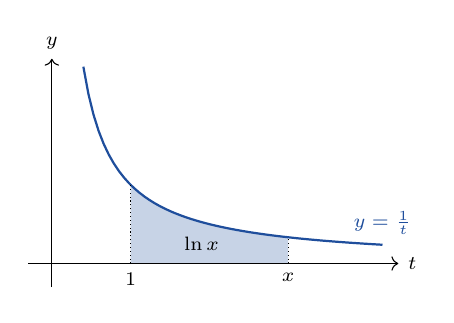
\begin{tikzpicture}[x=1cm,y=1cm,font=\scriptsize]
\fill[cDef!25] (1,0) -- plot[domain=1:3,samples=40] (\x,{1/\x}) -- (3,0) -- cycle;
\draw[->] (-0.3,0)--(4.4,0) node[right]{$t$}; \draw[->] (0,-0.3)--(0,2.6) node[above]{$y$};
\draw[cDef,thick,domain=0.4:4.2,samples=60] plot (\x,{1/\x}) node[above]{$y=\frac1t$};
\node[below] at (1,0){$1$}; \node[below] at (3,0){$x$}; \node at (1.9,0.25){$\ln x$};
\draw[densely dotted] (1,0)--(1,1) (3,0)--(3,0.333);
\end{tikzpicture}\end{LTR}\par (2) \underline{تعيين قيمة $\ln(1)$:} بالضغط على اللمسة \fbox{ln} ثم \fbox{1} ثم \fbox{=} نجد $\ln(1)=0$.\par (3) \underline{عبارة الدالة المشتقة:} نستنتج أن $\big[\ln(x)\big]^{\prime}=\dfrac1x$.\par (4) \underline{اتجاه تغير $\ln$:} بما أن $\dfrac1x>0$ على $]0;+\infty[$ فإن الدالة $\ln$ متزايدة تماماً على المجال $]0;+\infty[$.}{}{}
\Row{بناء المعارف}{%
\Lab{cDef}{تعريف}\ الدالة الوحيدة التي هي حل للتكامل $\displaystyle\int_1^x\dfrac1t\,dt$ تسمى \textbf{الدالة اللوغاريتمية النيبيرية} ونرمز لها بـ: $\ln$ ؛ مجموعة تعريفها $]0;+\infty[$.\par\Lab{cRem}{ملاحظات}\ نُشير إلى أن العدد $2{,}7182\dots$ نرمز له بـ $e$ ، مثل العدد الأصم $\pi$ الذي يساوي تقريباً $3{,}1415\dots$ ، ونكتب: $e\simeq2{,}7182\dots$ ؛ و $\ln(e)=1$.\par}{50 د}{إشارة $\ln x$ في جدول.}
\Row{}{%
\Lab{cThm}{مبرهنة}\par\ck\ $\ln(1)=0$ ؛ $\ln(e)=1$.\par
\ck\ الدالة $\ln$ قابلة للاشتقاق على $]0;+\infty[$ و $\big[\ln(x)\big]^{\prime}=\dfrac1x$.\par
\ck\ الدالة $\ln$ متزايدة تماماً على $]0;+\infty[$.\par
\ck\ من أجل $k>0$: $\big[\ln(kx)\big]^{\prime}=\dfrac k{kx}=\dfrac1x$.\par
\Lab{cRem}{إشارة $\ln(x)$}\ بما أن $\ln$ متزايدة تماماً و $\ln(1)=0$:\par\smallskip\begin{LTR}\centering {\footnotesize\renewcommand{\arraystretch}{1.45}\begin{tabular}{|c|ccccc|}\hline\rowcolor{cSec!12}$x$ & $0$ &  & $1$ &  & $+\infty$\\\hline $\ln(x)$ &  & $-$ & $0$ & $+$ & \\\hline \end{tabular}}\end{LTR}\par \ck\ $\ln(x)<0$ معناه $0<x<1$ ؛ $\ln(x)>0$ معناه $x>1$.\par
}{}{}
\Row{}{%
\Lab{cEx}{مثال 1}\ بالآلة الحاسبة: $\ln2\simeq0{,}69$ ، $\ln3\simeq1{,}10$ ، $\ln\dfrac12\simeq-0{,}69$ ، $\ln10\simeq2{,}30$.\par\Lab{cEx}{مثال 2}\ احسب المشتقة: $f(x)=3\ln x-2x$: $f^{\prime}(x)=\dfrac3x-2$ ؛ $g(x)=x\ln x$: $g^{\prime}(x)=\ln x+x\times\dfrac1x=\ln x+1$ ؛ $h(x)=\ln(5x)$: $h^{\prime}(x)=\dfrac1x$.}{}{}
\Row{التقويم}{%
\Lab{cMeth}{تمرين تطبيقي}\par $f$ الدالة المعرفة على $]0;+\infty[$ بـ: $f(x)=x-1-\ln x$.\par (1) احسب $f^{\prime}(x)$ ثم ادرس إشارتها. (2) شكّل جدول تغيرات $f$ (دون النهايات). (3) استنتج أن من أجل كل $x>0$: $\ln x\leqslant x-1$.\par}{25 د}{تقويم فردي.}
\Row{}{%
\Lab{cEx}{حل التمرين التطبيقي}\par (1) $f^{\prime}(x)=1-\dfrac1x=\dfrac{x-1}x$ ، إشارتها من إشارة $x-1$: سالبة على $]0;1[$ وموجبة على $]1;+\infty[$.\par\smallskip\begin{LTR}\centering 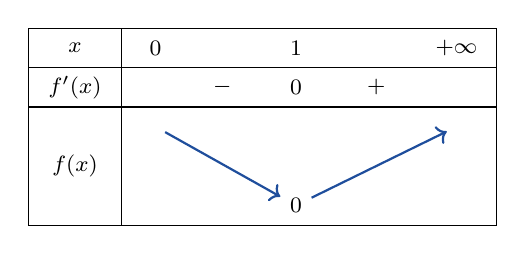
\begin{tikzpicture}[x=0.85cm,y=0.5cm,font=\footnotesize]
\draw (0,0) rectangle (7,-5); \draw (0,-1)--(7,-1); \draw (0,-2)--(7,-2); \draw (1.4,0)--(1.4,-5);
\node at (0.7,-0.5){$x$}; \node at (0.7,-1.5){$f^{\prime}(x)$}; \node at (0.7,-3.5){$f(x)$};
\node at (1.9,-0.5){$0$}; \node at (4,-0.5){$1$}; \node at (6.4,-0.5){$+\infty$};
\node at (2.9,-1.5){$-$}; \node at (4,-1.5){$0$}; \node at (5.2,-1.5){$+$};
\node (a) at (1.9,-2.5){$$}; \node (b) at (4,-4.5){$0$}; \node (c) at (6.4,-2.5){$$};
\draw[->,cDef,thick] (a)--(b); \draw[->,cDef,thick] (b)--(c);
\end{tikzpicture}\end{LTR}\par (3) القيمة الحدية الصغرى $f(1)=0$ ، إذن $f(x)\geqslant0$ أي $\ln x\leqslant x-1$.\par\textbf{واجب منزلي:} تمارين من الكتاب المدرسي صفحة 137.\par\smallskip\textbf{ملاحظات حول سير الحصة:} \dotfill}{}{}
\end{Sayr}
\newpage
\ModhHead{29}{3 ت ا}{تحليل}{الدالة اللوغاريتمية}{02 سا}{خواص الدالة اللوغاريتمية}%
{\begin{itemize}\item الدالة $\ln$ ومشتقتها ، $\big[\ln(kx)\big]^{\prime}=\frac1x$.\end{itemize}}%
{\begin{itemize}\item معرفة الخواص الجبرية للدالة اللوغاريتمية النيبيرية.\end{itemize}}%
{المنهاج ، الكتاب المدرسي ، الآلة الحاسبة ، برمجية Geogebra.}
\begin{Sayr}
\Row{مرحلة الانطلاق}{%
\textbf{التهيئة النفسية:} هل $\ln(2\times3)=\ln2\times\ln3$ ؟ تحقق بالآلة الحاسبة.}{10 د}{سؤال بالآلة الحاسبة.}
\Row{التشخيص والاكتشاف}{%
\Lab{cEx}{نشاط رقم 02}\ نعتبر الدالة $f$ المعرفة على $]0;+\infty[$ بـ: $f(x)=\ln(ax)-\ln(x)$ حيث $a$ عدد حقيقي موجب تماماً.\par (1) احسب $f^{\prime}(x)$ من أجل كل $x\in]0;+\infty[$. (2) احسب $f(1)$ ثم استنتج أن: $f(x)=\ln(a)$. (3) استنتج أن: $\ln(ab)=\ln(a)+\ln(b)$ من أجل كل $b\in]0;+\infty[$.\par\Lab{cDef}{مناقشة النشاط}\par (1) $f$ قابلة للاشتقاق على $]0;+\infty[$: $f^{\prime}(x)=\dfrac1x-\dfrac1x=0$ (لدينا من الدرس السابق: $\big[\ln(kx)\big]^{\prime}=\frac1x$).\par (2) $f(1)=\ln(a)-\ln(1)=\ln(a)$ ، وبما أن $f^{\prime}(x)=0$ فالدالة $f$ ثابتة أي $f(x)=f(1)$ ، وبالتالي $f(x)=\ln(a)$.\par (3) $\ln(ax)-\ln(x)=\ln(a)$ ، ومنه بوضع $x=b$: $\ln(ab)-\ln(b)=\ln(a)$ ، وبالتالي $\ln(ab)=\ln(a)+\ln(b)$.\par}{35 د}{الخاصية الأساسية من النشاط.}
\Row{}{%
\Lab{cRem}{ملاحظات}\ هذه الخاصية تُشير إلى أن اللوغاريتم النيبيري إذا دخل على الجداء يُحوّله إلى مجموع.}{}{}
\Row{بناء المعارف}{%
\Lab{cThm}{الخاصية الأساسية}\ من أجل كل عددين حقيقيين $x$ و $y$ من $]0;+\infty[$: $\ln(xy)=\ln(x)+\ln(y)$.\par\Lab{cEx}{مثال 1}\ $\ln(2e)=\ln2+\ln e=0{,}69+1=1{,}69$ ؛ $\ln(e^2)=\ln(e\times e)=\ln e+\ln e=2$.\par}{50 د}{كل خاصية ببرهانها ومثال.}
\Row{}{%
\Lab{cRem}{ملاحظة هامة}\ من أجل كل الأعداد الحقيقية الموجبة تماماً $a_1,a_2,\dots,a_n$: $\ln(a_1\times a_2\times\dots\times a_n)=\ln a_1+\ln a_2+\dots+\ln a_n$.\par\Lab{cEx}{مثال 2}\ احسب المجموع $S=\ln\left(\frac12\right)+\ln\left(\frac23\right)+\ln\left(\frac34\right)+\dots+\ln\left(\frac{99}{100}\right)$.\par لدينا: $S=\ln\left(\frac12\times\frac23\times\frac34\times\dots\times\frac{99}{100}\right)=\ln\left(\frac1{100}\right)$.\par}{}{}
\Row{}{%
\Lab{cThm}{الخاصية 02}\ من أجل كل $x\in]0;+\infty[$: $\ln\left(\dfrac1x\right)=-\ln(x)$.\par\Lab{cMeth}{البرهان}\ $0=\ln(1)=\ln\left(x\times\dfrac1x\right)=\ln(x)+\ln\left(\dfrac1x\right)$ ، ومنه $\ln\left(\dfrac1x\right)=-\ln(x)$.\par}{}{}
\Row{}{%
\Lab{cEx}{مثال 3}\ $\ln\left(\dfrac1e\right)=-\ln(e)=-1$.\par\Lab{cThm}{الخاصية 03}\ من أجل كل $x$ و $y$ من $]0;+\infty[$: $\ln\left(\dfrac xy\right)=\ln(x)-\ln(y)$.\par}{}{}
\Row{}{%
\Lab{cMeth}{البرهان}\ $\ln\left(\dfrac xy\right)=\ln\left(x\times\dfrac1y\right)=\ln(x)+\ln\left(\dfrac1y\right)=\ln(x)-\ln(y)$.\par\Lab{cEx}{مثال 4}\ بسّط العبارة $\ln\left(\dfrac{a^2-b^2}{a-b}\right)$ (مع $a>b>0$):\par $\ln\left(\dfrac{a^2-b^2}{a-b}\right)=\ln(a^2-b^2)-\ln(a-b)=\ln\big[(a-b)(a+b)\big]-\ln(a-b)=\ln(a+b)+\ln(a-b)-\ln(a-b)=\ln(a+b)$.\par}{}{}
\Row{}{%
\Lab{cThm}{الخاصية 04}\ من أجل كل $x\in]0;+\infty[$ ومن أجل كل عدد طبيعي $n$: $\ln(x^n)=n\times\ln(x)$.\par\Lab{cMeth}{البرهان}\ نبرهن بالتراجع:\par \underline{التحقق:} من أجل $n=0$: $\ln1=0\times\ln x$ (صحيحة).\par \underline{الفرضية:} نفرض أن $\ln(x^n)=n\ln(x)$ من أجل العدد الطبيعي $n$.\par \underline{الإثبات:} $\ln(x^{n+1})=\ln(x^n\times x)=\ln(x^n)+\ln(x)=n\ln(x)+\ln(x)=(n+1)\ln(x)$.\par وبالتالي حسب مبدأ البرهان بالتراجع: $\ln(x^n)=n\ln(x)$ من أجل كل عدد طبيعي $n$.\par}{}{}
\Row{}{%
\Lab{cEx}{مثال 5}\ من أجل كل عدد طبيعي $n$: $\ln(e^n)=n\times\ln(e)=n\times1=n$.\par\Lab{cRem}{ملاحظة هامة}\ نقبل تمديد الخاصية في المثال 5 ، أي من أجل كل عدد حقيقي $x$: $\ln(e^x)=x$.\par}{}{}
\Row{}{%
\Lab{cThm}{الخاصية 05}\ من أجل كل $x\in]0;+\infty[$: $\ln\left(\sqrt x\right)=\dfrac12\ln(x)$.\par\Lab{cMeth}{البرهان}\ $\ln(x)=\ln\left(\sqrt x^{\,2}\right)=2\ln\left(\sqrt x\right)$ ، ومنه $\ln\left(\sqrt x\right)=\dfrac12\ln(x)$.}{}{}
\Row{التقويم}{%
\Lab{cMeth}{تمرين تطبيقي}\ (متتالية عددية تتضمن اللوغاريتم النيبيري)\par $(u_n)_{n\in\mathbb N}$ متتالية عددية معرفة بحدها الأول $u_0=2$ وبالعلاقة التراجعية: $u_{n+1}=3u_n+4$ ، و $(v_n)_{n\in\mathbb N}$ معرفة بـ: $v_n=u_n+2$.\par (1) بيّن أن $(v_n)$ متتالية هندسية يطلب تعيين أساسها وحدها الأول. (2) اكتب عبارة $v_n$ بدلالة $n$ ثم استنتج عبارة $u_n$. (3) أ) احسب المجموع $S_n=v_0+v_1+\dots+v_n$. ب) عيّن العدد الطبيعي $n$ حتى يكون: $S_n=118096$. (4) $(w_n)$ معرفة بـ: $w_n=\ln(v_n)$: بيّن أن $(w_n)$ متتالية حسابية يطلب تعيين أساسها وحدها الأول ثم استنتج عبارة $w_n$ بدلالة $n$.\par}{25 د}{تقويم فردي.}
\Row{}{%
\Lab{cEx}{حل التمرين التطبيقي}\par (1) $v_{n+1}=u_{n+1}+2=3u_n+4+2=3u_n+6=3(u_n+2)=3v_n$: هندسية أساسها $q=3$ وحدها الأول $v_0=u_0+2=4$.\par (2) $v_n=v_0\times q^n=4\times3^n$ ؛ $u_n=v_n-2=4\times3^n-2$.\par (3) أ) $S_n=\dfrac{v_0}{1-q}\left(1-q^{n+1}\right)=\dfrac4{1-3}\left(1-3^{n+1}\right)=-2+6\times3^n$.\par ب) $-2+6\times3^n=118096$ معناه $3^n=19683$ ، أي $\ln(3^n)=\ln(19683)$ فيكون $n\ln3=\ln19683$ ، وبالتالي $n=\dfrac{\ln19683}{\ln3}=9$.\par (4) $w_{n+1}=\ln(v_{n+1})=\ln(3v_n)=\ln3+\ln(v_n)=\ln3+w_n$: حسابية أساسها $r=\ln3$ وحدها الأول $w_0=\ln(v_0)=\ln4$ ؛ فيكون $w_n=w_0+nr=\ln4+n\ln3$.\par\textbf{واجب منزلي:} تمارين من الكتاب المدرسي صفحة 137.\par\smallskip\textbf{ملاحظات حول سير الحصة:} \dotfill}{}{}
\end{Sayr}
\newpage
\ModhHead{30}{3 ت ا}{تحليل}{الدالة اللوغاريتمية}{02 سا}{معادلات ومتراجحات لوغاريتمية}%
{\begin{itemize}\item خواص الدالة $\ln$ ، اتجاه تغيرها ، المعادلات من الدرجة الثانية.\end{itemize}}%
{\begin{itemize}\item حل معادلات ومتراجحات تتضمن اللوغاريتم النيبيري.\end{itemize}}%
{المنهاج ، الكتاب المدرسي ، الآلة الحاسبة ، برمجية Geogebra.}
\begin{Sayr}
\Row{مرحلة الانطلاق}{%
\textbf{التهيئة النفسية:} إذا كان $\ln a=\ln b$ ، هل يكون $a=b$ ؟ لماذا؟}{10 د}{سؤال.}
\Row{التشخيص والاكتشاف}{%
\Lab{cEx}{نشاط رقم 03}\ (1) حُل في $\mathbb R$ المعادلة: $\ln(x^2-1)=\ln(x+5)\ \dots(\clubsuit)$. (2) حُل في $\mathbb R$ المتراجحة: $\ln(x^2-1)<\ln(x+5)\ \dots(\spadesuit)$.\par\Lab{cDef}{مناقشة النشاط}\par (1) \underline{حل المعادلة $(\clubsuit)$:} معرفة على $D=\{x\in\mathbb R\ /\ x+5>0\ \text{\ar{و}}\ x^2-1>0\}$.\par $x^2-1>0$ معناه $x^2>1$ أي $|x|>1$: $x>1$ أو $x<-1$ ، فيكون $D_1=]-\infty;-1[\cup]1;+\infty[$ ؛ $x+5>0$ معناه $x>-5$: $D_2=]-5;+\infty[$. وبالتالي $D=D_1\cap D_2$:\par\smallskip\begin{LTR}\centering 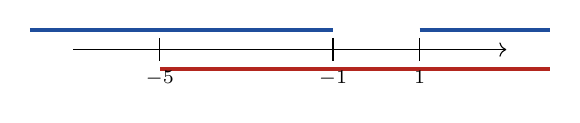
\begin{tikzpicture}[x=0.55cm,font=\scriptsize] \draw[->] (-7,0)--(3,0);\draw[cDef,line width=1.6pt] (-8,0.25)--(-1,0.25);\draw[cDef,line width=1.6pt] (1,0.25)--(4,0.25);\draw[cThm,line width=1.6pt] (-5,-0.25)--(4,-0.25);\draw (-5,0.15)--(-5,-0.15) node[below]{$-5$};\draw (-1,0.15)--(-1,-0.15) node[below]{$-1$};\draw (1,0.15)--(1,-0.15) node[below]{$1$};\end{tikzpicture}\end{LTR}\par فيكون: $D=]-5;-1[\cup]1;+\infty[$.\par $(\clubsuit)$ تكافئ $x^2-1=x+5$ ومنه $x^2-x-6=0$ ، $\Delta=25$: $x_1=3$ و $x_2=-2$ ، وبما أن $3\in D$ و $-2\in D$ فإن: $S=\{-2;3\}$.\par (2) \underline{حل المتراجحة $(\spadesuit)$:} معرفة على $D$ ، وتكافئ $x^2-1<x+5$ ومنه $x^2-x-6<0$:\par\smallskip\begin{LTR}\centering {\footnotesize\renewcommand{\arraystretch}{1.45}\begin{tabular}{|c|ccccccc|}\hline\rowcolor{cSec!12}$x$ & $-\infty$ &  & $-2$ &  & $3$ &  & $+\infty$\\\hline $x^2-x-6$ &  & $+$ & $0$ & $-$ & $0$ & $+$ & \\\hline \end{tabular}}\end{LTR}\par أي $x\in]-2;3[$ وبالتالي $S^{\prime}=]-2;3[\cap D$:\par\smallskip\begin{LTR}\centering 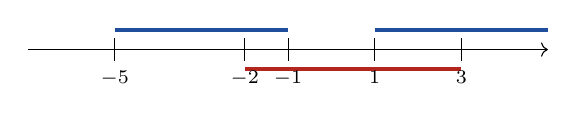
\begin{tikzpicture}[x=0.55cm,font=\scriptsize] \draw[->] (-7,0)--(5,0);\draw[cDef,line width=1.6pt] (-5,0.25)--(-1,0.25);\draw[cDef,line width=1.6pt] (1,0.25)--(5,0.25);\draw[cThm,line width=1.6pt] (-2,-0.25)--(3,-0.25);\draw (-5,0.15)--(-5,-0.15) node[below]{$-5$};\draw (-2,0.15)--(-2,-0.15) node[below]{$-2$};\draw (-1,0.15)--(-1,-0.15) node[below]{$-1$};\draw (1,0.15)--(1,-0.15) node[below]{$1$};\draw (3,0.15)--(3,-0.15) node[below]{$3$};\end{tikzpicture}\end{LTR}\par فيكون: $S^{\prime}=]-2;-1[\cup]1;3[$.}{35 د}{نستعين بالمستقيم العددي لتقاطع المجالين.}
\Row{بناء المعارف}{%
\Lab{cThm}{مبرهنة}\ من أجل $a$ و $b$ عددين حقيقيين موجبين تماماً:\par\ck\ $\ln(a)=\ln(b)$ معناه $a=b$.\par
\ck\ $\ln(a)\leqslant\ln(b)$ معناه $a\leqslant b$.\par
\Lab{cMeth}{البرهان}\ من جدول تغيرات الدالة $\ln$ (متزايدة تماماً على $]0;+\infty[$) نستنتج العلاقتين السابقتين.\par}{50 د}{مجموعة التعريف أولاً.}
\Row{}{%
\Lab{cEx}{مثال 1}\ حل في $D=]-1;+\infty[$ المعادلة: $\ln(x+1)=4\ \dots(\bigstar)$.\par نعلم أن $4=\ln e^4$ ومنه $(\bigstar)$ تكافئ $\ln(x+1)=\ln e^4$ وبالتالي $x+1=e^4$ ، فيكون $x=e^4-1$ ، وبما أن $e^4-1\in D$ فإن: $S=\{e^4-1\}$.\par\Lab{cEx}{مثال 2}\ حل في $D=]3;+\infty[$ المتراجحة: $\ln(x-3)\leqslant0\ \dots(\blacktriangle)$.\par نعلم أن $\ln1=0$ وبالتالي $(\blacktriangle)$ تكافئ $\ln(x-3)\leqslant\ln1$ ومنه $x-3\leqslant1$ أي $x\leqslant4$ ؛ وعليه $S=]-\infty;4]\cap D$:\par\smallskip\begin{LTR}\centering 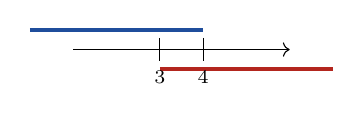
\begin{tikzpicture}[x=0.55cm,font=\scriptsize] \draw[->] (1,0)--(6,0);\draw[cDef,line width=1.6pt] (0,0.25)--(4,0.25);\draw[cThm,line width=1.6pt] (3,-0.25)--(7,-0.25);\draw (3,0.15)--(3,-0.15) node[below]{$3$};\draw (4,0.15)--(4,-0.15) node[below]{$4$};\end{tikzpicture}\end{LTR}\par فيكون: $S=]3;4]$.\par}{}{}
\Row{}{%
\Lab{cRem}{ملاحظة هامة}\ لحل معادلة من الشكل $\ln\big[u(x)\big]=\ln\big[v(x)\big]$ أو متراجحة من الشكل $\ln\big[u(x)\big]<\ln\big[v(x)\big]$: (1) نعيّن $D$ مجموعة تعريف المعادلة أو المتراجحة. (2) نحل في $D$ المعادلة $u(x)=v(x)$ أو المتراجحة $u(x)<v(x)$.\par\Lab{cEx}{مثال 3}\ حل في $D=]-2;+\infty[$ المتراجحة: $\ln(x+2)+\ln(x+3)\leqslant\ln(6)\ \dots(\heartsuit)$.\par من أجل كل $x\in D$ المتراجحة $(\heartsuit)$ تكافئ $\ln\big[(x+2)(x+3)\big]\leqslant\ln6$ ، معناه $(x+2)(x+3)\leqslant6$ أي $x^2+5x\leqslant0$:\par\smallskip\begin{LTR}\centering {\footnotesize\renewcommand{\arraystretch}{1.45}\begin{tabular}{|c|ccccccc|}\hline\rowcolor{cSec!12}$x$ & $-\infty$ &  & $-5$ &  & $0$ &  & $+\infty$\\\hline $x^2+5x$ &  & $+$ & $0$ & $-$ & $0$ & $+$ & \\\hline \end{tabular}}\end{LTR}\par وبالتالي $S=[-5;0]\cap D$ ، فيكون: $S=]-2;0]$.}{}{}
\Row{التقويم}{%
\Lab{cMeth}{تمرين تطبيقي}\ (بكالوريا 2024 ، الموضوع الثاني ، شعبة تسيير واقتصاد)\par $P$ الدالة المعرفة على $\mathbb R$ بـ: $P(X)=(2X-1)(X^2+X-2)$.\par (1) ادرس إشارة $P(X)$ حسب قيم $X$ من $\mathbb R$. (2) أ) حل في $]0;+\infty[$ المعادلة: $(2\ln x-1)\big((\ln x)^2+\ln x-2\big)=0$. ب) استنتج في $]0;+\infty[$ حلول المتراجحة: $(2\ln x-1)\big((\ln x)^2+\ln x-2\big)<0$. (3) حُل في $]-1;+\infty[$ المعادلة: $\big(\ln(x+1)\big)^2+\ln(x+1)-2=0$.\par}{25 د}{تقويم فردي.}
\Row{}{%
\Lab{cEx}{حل التمرين التطبيقي}\par (1) $X^2+X-2=(X-1)(X+2)$:\par\smallskip\begin{LTR}\centering {\footnotesize\renewcommand{\arraystretch}{1.45}\begin{tabular}{|c|ccccccccc|}\hline\rowcolor{cSec!12}$x$ & $-\infty$ &  & $-2$ &  & $\frac12$ &  & $1$ &  & $+\infty$\\\hline $2X-1$ &  & $-$ &  & $-$ & $0$ & $+$ &  & $+$ & \\\hline $X^2+X-2$ &  & $+$ & $0$ & $-$ &  & $-$ & $0$ & $+$ & \\\hline $P(X)$ &  & $-$ & $0$ & $+$ & $0$ & $-$ & $0$ & $+$ & \\\hline \end{tabular}}\end{LTR}\par }{}{}
\Row{}{%
\Lab{cEx}{تابع الحل}\ (2) أ) بوضع $X=\ln(x)$ نحصل على المعادلة $P\big(\ln(x)\big)=0$ ، وبالتالي:\par\ck\ $X=-2$: $\ln(x)=-2=\ln e^{-2}$ أي $x=e^{-2}$.\par
\ck\ $X=\frac12$: $\ln(x)=\frac12=\ln\sqrt e$ أي $x=\sqrt e$.\par
\ck\ $X=1$: $\ln(x)=1=\ln e$ أي $x=e$.\par
وبما أن $e^{-2}$ ، $\sqrt e$ ، $e$ تنتمي إلى $]0;+\infty[$ فإن: $S=\{e^{-2};\sqrt e;e\}$.\par}{}{}
\Row{}{%
\Lab{cEx}{تابع الحل}\ ب) بوضع $X=\ln(x)$ يصبح لدينا:\par\smallskip\begin{LTR}\centering {\footnotesize\renewcommand{\arraystretch}{1.45}\begin{tabular}{|c|ccccccccc|}\hline\rowcolor{cSec!12}$x$ & $0$ &  & $e^{-2}$ &  & $\sqrt e$ &  & $e$ &  & $+\infty$\\\hline $P(\ln x)$ &  & $-$ & $0$ & $+$ & $0$ & $-$ & $0$ & $+$ & \\\hline \end{tabular}}\end{LTR}\par وبالتالي حلول المتراجحة $P(\ln x)<0$ هي: $S^{\prime}=]0;e^{-2}[\cup]\sqrt e;e[$.\par (3) بوضع $X=\ln(x+1)$: $X^2+X-2=0$ ، $X=1$ أو $X=-2$.\par\ck\ $\ln(x+1)=1=\ln e$: $x+1=e$ وبالتالي $x=e-1$.\par
\ck\ $\ln(x+1)=-2=\ln e^{-2}$: $x+1=e^{-2}$ وبالتالي $x=e^{-2}-1$.\par
بما أن $e-1$ و $e^{-2}-1$ ينتميان إلى $]-1;+\infty[$: $S^{\prime\prime}=\{e^{-2}-1;e-1\}$.\par\textbf{واجب منزلي:} تمارين من الكتاب المدرسي صفحة 137.\par\smallskip\textbf{ملاحظات حول سير الحصة:} \dotfill}{}{}
\end{Sayr}
\newpage
\ModhHead{31}{3 ت ا}{تحليل}{الدالة اللوغاريتمية}{02 سا}{دراسة الدالة اللوغاريتمية النيبيرية}%
{\begin{itemize}\item خواص $\ln$ ، النهايات ، مبرهنة القيم المتوسطة ، معادلة المماس.\end{itemize}}%
{\begin{itemize}\item الدراسة والتمثيل البياني للدالة اللوغاريتمية النيبيرية.\item دراسة النتائج المتعلقة بالنهايات الشهيرة.\end{itemize}}%
{المنهاج ، الكتاب المدرسي ، الآلة الحاسبة ، برمجية Geogebra.}
\begin{Sayr}
\Row{مرحلة الانطلاق}{%
\textbf{التهيئة النفسية:} ما سلوك منحنى $\ln$ عند طرفي مجال تعريفه؟}{10 د}{Geogebra.}
\Row{التشخيص والاكتشاف}{%
\Lab{cEx}{نشاط رقم 04}\ باستعمال برمجية Geogebra مثّلنا منحنى الدالة $\ln$. (1) خمّن نهاية الدالة $\ln$ لما $x$ يؤول إلى $+\infty$. (2) خمّن: $\lim\limits_{x\to 0}\ln(x)$ ثم فسّر النتيجة هندسياً.\par\Lab{cDef}{مناقشة النشاط}\par (1) نُخمّن أن: $\lim\limits_{x\to +\infty}\ln(x)=+\infty$. (2) نُخمّن أن: $\lim\limits_{x\to 0}\ln(x)=-\infty$ ؛ \underline{التفسير الهندسي:} منحنى الدالة $\ln$ يقبل محور التراتيب كمستقيم مقارب.\par}{35 د}{التخمين ثم المبرهنة.}
\Row{}{%
\Lab{cRem}{ملاحظات}\ بقراءة بيانية يمكن تخمين نهايتي الدالة $\ln$ عند طرفي مجال تعريفها.}{}{}
\Row{بناء المعارف}{%
\Lab{cDef}{1. النهايات}\par\Lab{cThm}{تُقبل بدون برهان}\ $\lim\limits_{x\to +\infty}\ln(x)=+\infty$.\par}{50 د}{جدول القيم والرسم.}
\Row{}{%
\Lab{cEx}{مثال 1}\ $\lim\limits_{x\to +\infty}\left(x^2-1+2\ln x\right)=+\infty$ و $\lim\limits_{x\to +\infty}\left(1-\ln x-x\right)=-\infty$.\par\Lab{cThm}{مبرهنة}\ $\lim\limits_{\substack{x\to0\\x>0}}\ln(x)=-\infty$.\par}{}{}
\Row{}{%
\Lab{cMeth}{البرهان}\ بوضع $X=\dfrac1x$: $\lim\limits_{\substack{x\to0\\x>0}}\ln x=\lim\limits_{X\to+\infty}\ln\left(\dfrac1X\right)=\lim\limits_{X\to+\infty}\big(-\ln X\big)=-\infty$.\par\Lab{cEx}{مثال 2}\ $\lim\limits_{\substack{x\to0\\x>0}}\dfrac{1+\ln x}{1-\ln x}=\lim\limits_{\substack{x\to0\\x>0}}\dfrac{\ln x\left(\frac1{\ln x}+1\right)}{\ln x\left(\frac1{\ln x}-1\right)}=\lim\limits_{\substack{x\to0\\x>0}}\dfrac{\frac1{\ln x}+1}{\frac1{\ln x}-1}=-1$.\par}{}{}
\Row{}{%
\Lab{cDef}{2. التمثيل البياني}\ نُعرّف الدالة $\ln$ بجدول القيم التالي:\par\smallskip\begin{LTR}\centering {\footnotesize\renewcommand{\arraystretch}{1.6}\begin{tabular}{|c|c|c|c|c|c|c|c|}\hline\rowcolor{cSec!12}$x$ & $\frac14$ & $\frac13$ & $\frac12$ & $1$ & $2$ & $e$ & $e^2$\\\hline $\ln(x)$ & $-1{,}39$ & $-1{,}10$ & $-0{,}69$ & $0$ & $0{,}69$ & $1$ & $2$\\\hline\end{tabular}}\end{LTR}\par \par\smallskip\begin{LTR}\centering 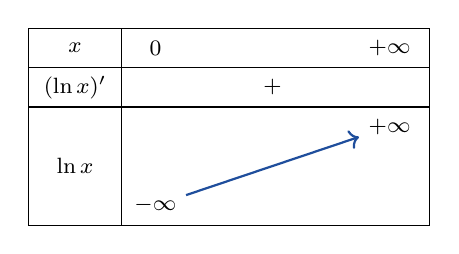
\begin{tikzpicture}[x=0.85cm,y=0.5cm,font=\footnotesize]
\draw (0,0) rectangle (6,-5); \draw (0,-1)--(6,-1); \draw (0,-2)--(6,-2); \draw (1.4,0)--(1.4,-5);
\node at (0.7,-0.5){$x$}; \node at (0.7,-1.5){$(\ln x)^{\prime}$}; \node at (0.7,-3.5){$\ln x$};
\node at (1.9,-0.5){$0$}; \node at (5.4,-0.5){$+\infty$}; \node at (3.65,-1.5){$+$};
\node (a) at (1.9,-4.5){$-\infty$}; \node (c) at (5.4,-2.5){$+\infty$}; \draw[->,cDef,thick] (a)--(c);
\end{tikzpicture}\end{LTR}\par \par\smallskip\begin{LTR}\centering 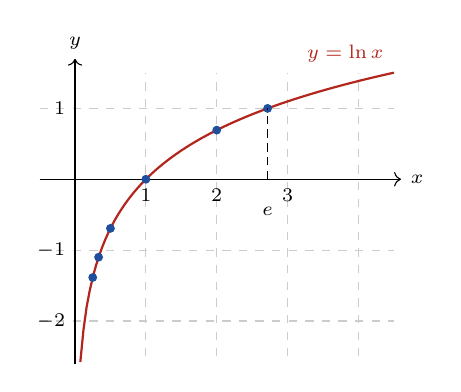
\begin{tikzpicture}[x=0.9cm,y=0.9cm,font=\scriptsize]
\draw[gray!40,dashed,step=1] (-0.5,-2.5) grid (4.5,1.5);
\draw[->] (-0.5,0)--(4.6,0) node[right]{$x$}; \draw[->] (0,-2.6)--(0,1.7) node[above]{$y$};
\foreach \t in {1,2,3} \node[below] at (\t,0){$\t$}; \foreach \t in {-2,-1,1} \node[left] at (0,\t){$\t$};
\draw[cThm,thick,domain=0.075:4.5,samples=100] plot (\x,{ln(\x)}) node[above left]{$y=\ln x$};
\foreach \p in {0.25,0.333,0.5,1,2,2.718} \fill[cDef] (\p,{ln(\p)}) circle (1.6pt);
\draw[densely dashed] (2.718,0)--(2.718,1); \node[below] at (2.718,-0.25){$e$};
\end{tikzpicture}\end{LTR}\par التمثيل البياني للدالة $\ln$ يقبل محور التراتيب كمستقيم مقارب.\par\Lab{cDef}{3. العدد أولر}\ الدالة $\ln$ مستمرة ومتزايدة تماماً على $]0;+\infty[$ و $\lim\limits_{x\to 0^{+}}\ln x<1<\lim\limits_{x\to +\infty}\ln x$ ، وبالتالي حسب مبرهنة القيم المتوسطة ورتابة $\ln$ المعادلة $\ln x=1$ تقبل حلاً وحيداً يسمى العدد أولر ونرمز له بـ $e$ حيث $e\simeq2{,}7182\dots$\par}{}{}
\Row{}{%
\Lab{cDef}{4. معادلة المماس}\par\Lab{cThm}{مبرهنة}\ المستقيم $(\Delta)$ ذو المعادلة $y=x-1$ مماس لمنحنى الدالة $\ln$ عند النقطة التي فاصلتها $1$.\par}{}{}
\Row{}{%
\Lab{cMeth}{البرهان}\ $y=\ln^{\prime}(1)(x-1)+\ln(1)$ حيث $\ln(1)=0$ و $\ln^{\prime}(1)=\frac11=1$ ، وبالتالي $(\Delta):y=x-1$ ، وهو أحسن تقريب تآلفي للدالة $\ln$ بجوار $1$.}{}{}
\Row{التقويم}{%
\Lab{cMeth}{تمرين تطبيقي}\ (بكالوريا 2020 ، الموضوع الأول ، شعبة تسيير واقتصاد)\par \textbf{I.} $g(x)=x^2-1+\ln x$ على $]0;+\infty[$. (1) احسب $\lim\limits_{x\to 0^{+}}g(x)$ و $\lim\limits_{x\to +\infty}g(x)$. (2) ادرس اتجاه تغير $g$ ثم شكّل جدول تغيراتها. (3) احسب $g(1)$ ثم استنتج إشارة $g(x)$.\par \textbf{II.} $f(x)=\frac13x^3-2x+2+x\ln x$ على $]0;+\infty[$ و $(\mathcal C_f)$ تمثيلها البياني. (1) احسب $\lim\limits_{x\to 0^{+}}f(x)$ و $\lim\limits_{x\to +\infty}f(x)$ (يُعطى: $\lim\limits_{x\to 0^{+}}x\ln x=0$). (2) بيّن أن $f^{\prime}(x)=g(x)$. (3) استنتج اتجاه تغير $f$ ثم شكّل جدول تغيراتها. (4) احسب $f(2)$ ثم أنشئ $(\mathcal C_f)$. (5) $F(x)=\frac1{12}x^4-\frac54x^2+2x-8+\frac12x^2\ln x$: بيّن أن $F$ دالة أصلية لـ $f$ على $]0;+\infty[$.\par}{25 د}{تمرينا بكالوريا: حل جماعي ثم فردي.}
\Row{}{%
\Lab{cEx}{حل التمرين التطبيقي}\par \textbf{I.} (1) $\lim\limits_{x\to 0^{+}}g(x)=-\infty$ ؛ $\lim\limits_{x\to +\infty}g(x)=+\infty$. (2) $g^{\prime}(x)=2x+\dfrac1x=\dfrac{2x^2+1}x>0$: $g$ متزايدة تماماً على $]0;+\infty[$.\par\smallskip\begin{LTR}\centering 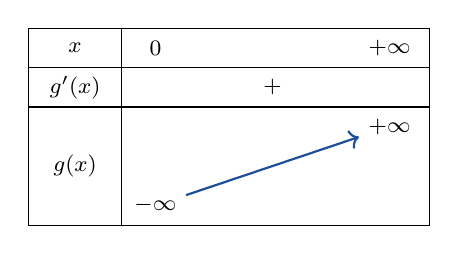
\begin{tikzpicture}[x=0.85cm,y=0.5cm,font=\footnotesize]
\draw (0,0) rectangle (6,-5); \draw (0,-1)--(6,-1); \draw (0,-2)--(6,-2); \draw (1.4,0)--(1.4,-5);
\node at (0.7,-0.5){$x$}; \node at (0.7,-1.5){$g^{\prime}(x)$}; \node at (0.7,-3.5){$g(x)$};
\node at (1.9,-0.5){$0$}; \node at (5.4,-0.5){$+\infty$}; \node at (3.65,-1.5){$+$};
\node (a) at (1.9,-4.5){$-\infty$}; \node (c) at (5.4,-2.5){$+\infty$}; \draw[->,cDef,thick] (a)--(c);
\end{tikzpicture}\end{LTR}\par (3) $g(1)=1^2-1+\ln1=0$:\par\smallskip\begin{LTR}\centering {\footnotesize\renewcommand{\arraystretch}{1.45}\begin{tabular}{|c|ccccc|}\hline\rowcolor{cSec!12}$x$ & $0$ &  & $1$ &  & $+\infty$\\\hline $g(x)$ &  & $-$ & $0$ & $+$ & \\\hline \end{tabular}}\end{LTR}\par }{}{}
\Row{}{%
\Lab{cEx}{حل الجزء II}\ (1) $\lim\limits_{x\to 0^{+}}f(x)=2$ ؛ $\lim\limits_{x\to +\infty}f(x)=+\infty$. (2) $f^{\prime}(x)=x^2-2+\ln x+x\times\dfrac1x=x^2-1+\ln x=g(x)$.\par (3) إشارة $f^{\prime}(x)$ من إشارة $g(x)$: $f$ متناقصة تماماً على $]0;1]$ ومتزايدة تماماً على $[1;+\infty[$.\par\smallskip\begin{LTR}\centering 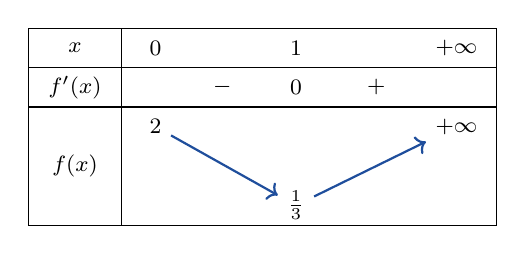
\begin{tikzpicture}[x=0.85cm,y=0.5cm,font=\footnotesize]
\draw (0,0) rectangle (7,-5); \draw (0,-1)--(7,-1); \draw (0,-2)--(7,-2); \draw (1.4,0)--(1.4,-5);
\node at (0.7,-0.5){$x$}; \node at (0.7,-1.5){$f^{\prime}(x)$}; \node at (0.7,-3.5){$f(x)$};
\node at (1.9,-0.5){$0$}; \node at (4,-0.5){$1$}; \node at (6.4,-0.5){$+\infty$};
\node at (2.9,-1.5){$-$}; \node at (4,-1.5){$0$}; \node at (5.2,-1.5){$+$};
\node (a) at (1.9,-2.5){$2$}; \node (b) at (4,-4.5){$\frac13$}; \node (c) at (6.4,-2.5){$+\infty$};
\draw[->,cDef,thick] (a)--(b); \draw[->,cDef,thick] (b)--(c);
\end{tikzpicture}\end{LTR}\par }{}{}
\Row{}{%
\Lab{cEx}{تابع الحل}\ (4) $f(2)=\frac13(2)^3-2(2)+2+2\ln2\simeq2{,}05$.\par\smallskip\begin{LTR}\centering 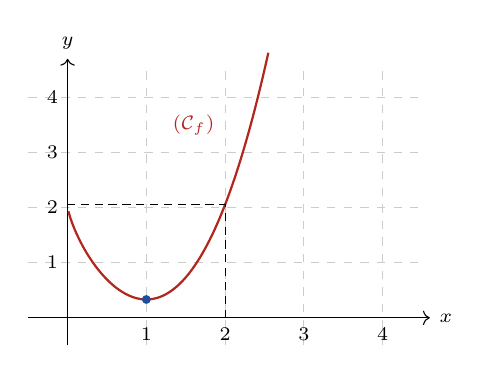
\begin{tikzpicture}[x=1cm,y=0.7cm,font=\scriptsize]
\draw[gray!40,dashed,step=1] (-0.5,-0.5) grid (4.5,4.5);
\draw[->] (-0.5,0)--(4.6,0) node[right]{$x$}; \draw[->] (0,-0.5)--(0,4.7) node[above]{$y$};
\foreach \t in {1,2,3,4} {\node[below] at (\t,0){$\t$}; \node[left] at (0,\t){$\t$};}
\draw[cThm,thick,domain=0.01:2.55,samples=100] plot (\x,{\x*\x*\x/3-2*\x+2+\x*ln(\x)}); \node[cThm] at (1.6,3.5){$(\mathcal C_f)$};
\fill[cDef] (1,0.333) circle (1.6pt); \draw[densely dashed] (2,0)--(2,2.05)--(0,2.05);
\end{tikzpicture}\end{LTR}\par (5) $F^{\prime}(x)=\frac13x^3-\frac52x+2+\frac12\left(2x\ln x+x^2\times\frac1x\right)=\frac13x^3-\frac52x+2+x\ln x+\frac12x=\frac13x^3-2x+2+x\ln x=f(x)$.}{}{}
\Row{}{%
\Lab{cMeth}{تمرين تطبيقي}\ (بكالوريا 2018 ، الموضوع الأول ، شعبة تسيير واقتصاد)\par $f(x)=\ln(x+2)+\ln(-x+8)-\ln16$ على $]-2;8[$ ، والوحدة البيانية $2\,\text{cm}$. (1) احسب نهايتي $f$ عند طرفي مجموعة التعريف وفسّر النتيجتين بيانياً. (2) تحقق أن $f^{\prime}(x)=\dfrac{-2x+6}{(x+2)(-x+8)}$. (3) ادرس إشارة $f^{\prime}(x)$ وشكّل جدول تغيرات $f$. (4) عيّن نقط تقاطع $(\mathcal C_f)$ مع محوري الإحداثيات. (5) بيّن أن من أجل كل $x\in]-2;8[$: $6-x\in]-2;8[$ و $f(6-x)=f(x)$ ثم فسّر النتيجة بيانياً. (6) ارسم $(\mathcal C_f)$. (7) بيّن أن $F(x)=(x+2)\ln(x+2)+(x-8)\ln(-x+8)-2x-x\ln16$ دالة أصلية لـ $f$ على $]-2;8[$. (8) احسب بـ $\text{cm}^2$ مساحة الحيز المحدد بـ $(\mathcal C_f)$ والمستقيمات $y=0$ ، $x=0$ و $x=4$.\par}{}{}
\Row{}{%
\Lab{cEx}{حل التمرين التطبيقي}\par (1) $\lim\limits_{x\to -2^{+}}f(x)=-\infty$ و $\lim\limits_{x\to 8^{-}}f(x)=-\infty$: $(\mathcal C_f)$ يقبل مستقيمين مقاربين عموديين معادلتاهما $x=-2$ و $x=8$.\par (2) $f^{\prime}(x)=\dfrac1{x+2}-\dfrac1{8-x}=\dfrac{8-x-x-2}{(x+2)(8-x)}=\dfrac{-2x+6}{(x+2)(8-x)}$.\par (3) $(x+2)(8-x)>0$ على $]-2;8[$ ، فإشارة $f^{\prime}(x)$ من إشارة $-2x+6$:\par\smallskip\begin{LTR}\centering 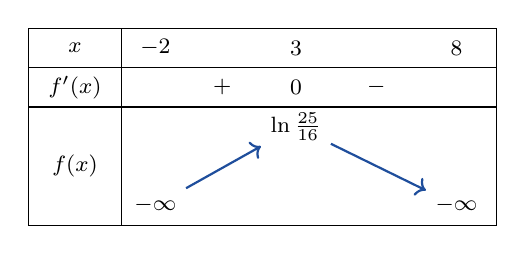
\begin{tikzpicture}[x=0.85cm,y=0.5cm,font=\footnotesize]
\draw (0,0) rectangle (7,-5); \draw (0,-1)--(7,-1); \draw (0,-2)--(7,-2); \draw (1.4,0)--(1.4,-5);
\node at (0.7,-0.5){$x$}; \node at (0.7,-1.5){$f^{\prime}(x)$}; \node at (0.7,-3.5){$f(x)$};
\node at (1.9,-0.5){$-2$}; \node at (4,-0.5){$3$}; \node at (6.4,-0.5){$8$};
\node at (2.9,-1.5){$+$}; \node at (4,-1.5){$0$}; \node at (5.2,-1.5){$-$};
\node (a) at (1.9,-4.5){$-\infty$}; \node (b) at (4,-2.5){$\ln\frac{25}{16}$}; \node (c) at (6.4,-4.5){$-\infty$};
\draw[->,cDef,thick] (a)--(b); \draw[->,cDef,thick] (b)--(c);
\end{tikzpicture}\end{LTR}\par }{}{}
\Row{}{%
\Lab{cEx}{تابع الحل}\ (4) \underline{مع محور الفواصل:} $f(x)=0$ معناه $\ln\dfrac{(x+2)(8-x)}{16}=\ln1$ ، أي $(x+2)(8-x)=16$ ، يكافئ $-x^2+6x=0$: $x=0$ أو $x=6$ (ينتميان إلى $]-2;8[$): النقطتان $O(0;0)$ و $A(6;0)$. \underline{مع محور التراتيب:} $f(0)=\ln2+\ln8-\ln16=0$: النقطة $O(0;0)$.\par (5) $-2<x<8$ معناه $-8<-x<2$ ، ثم بإضافة $6$: $-2<6-x<8$. و $f(6-x)=\ln(8-x)+\ln(2+x)-\ln16=f(x)$: $(\mathcal C_f)$ يقبل محور تناظر معادلته $x=3$.\par (6) الرسم (الحيز الملوّن للسؤال 8):\par\smallskip\begin{LTR}\centering 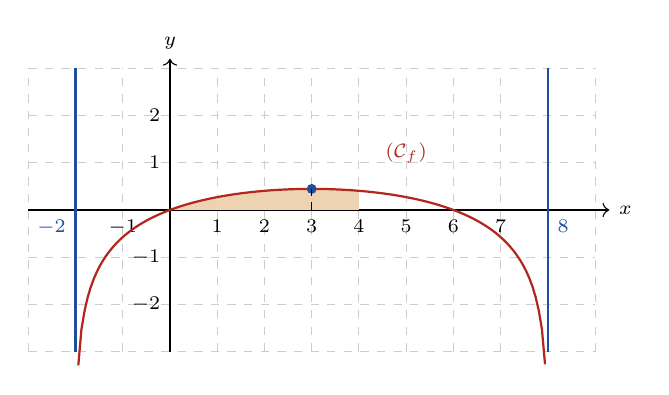
\begin{tikzpicture}[x=0.6cm,y=0.6cm,font=\scriptsize]
\draw[gray!40,dashed,step=1] (-3,-3) grid (9,3);
\draw[->] (-3,0)--(9.3,0) node[right]{$x$}; \draw[->] (0,-3)--(0,3.2) node[above]{$y$};
\foreach \t in {-1,1,2,3,4,5,6,7} \node[below] at (\t,0){$\t$}; \foreach \t in {-2,-1,1,2} \node[left] at (0,\t){$\t$};
\draw[cDef,thick] (-2,-3)--(-2,3) (8,-3)--(8,3); \node[cDef,below left] at (-2,0){$-2$}; \node[cDef,below right] at (8,0){$8$};
\fill[cEx!30] (0,0) -- plot[domain=0:4,samples=40] (\x,{ln(\x+2)+ln(8-\x)-ln(16)}) -- (4,0) -- cycle;
\draw[cThm,thick,domain=-1.94:7.94,samples=150] plot (\x,{ln(\x+2)+ln(8-\x)-ln(16)}); \node[cThm] at (5,1.2){$(\mathcal C_f)$};
\fill[cDef] (3,0.446) circle (1.8pt); \draw[densely dashed] (3,0)--(3,0.446);
\end{tikzpicture}\end{LTR}\par }{}{}
\Row{}{%
\Lab{cEx}{تابع الحل}\ (7) $F^{\prime}(x)=\ln(x+2)+\dfrac{x+2}{x+2}+\ln(-x+8)+\dfrac{8-x}{8-x}-2-\ln16=\ln(x+2)+\ln(-x+8)-\ln16=f(x)$.\par (8) على $[0;4]$: $f(x)\geqslant0$ (من جدول التغيرات و $f(0)=0$):\par\smallskip\begin{LTR}\centering {\footnotesize\renewcommand{\arraystretch}{1.45}\begin{tabular}{|c|ccc|}\hline\rowcolor{cSec!12}$x$ & $0$ &  & $4$\\\hline $f(x)$ & $0$ & $+$ & \\\hline \ar{الوضع النسبي} &  & \ar{$(\mathcal C_f)$ فوق $(xx^{\prime})$} & \\\hline \end{tabular}}\end{LTR}\par $\mathcal A=4\,\text{cm}^2\times\displaystyle\int_0^4f(x)\,dx=4\big(F(4)-F(0)\big)=4\big(6\ln6-4\ln4-8-4\ln16-2\ln2+8\ln8\big)\simeq5{,}457\,\text{cm}^2$.\par\textbf{واجب منزلي:} تمارين من صفحة 143 إلى 147.\par\smallskip\textbf{ملاحظات حول سير الحصة:} \dotfill}{}{}
\end{Sayr}
\newpage
\ModhHead{32}{3 ت ا}{تحليل}{الدالة اللوغاريتمية}{02 سا}{نهايات دوال لوغاريتمية}%
{\begin{itemize}\item دراسة الدالة $\ln$ ، النهايات بالمقارنة.\end{itemize}}%
{\begin{itemize}\item معرفة وتفسير النهايات الشهيرة.\item حساب نهايات جداءات أو حواصل قسمة تتضمن $x$ و $\ln(x)$.\end{itemize}}%
{المنهاج ، الكتاب المدرسي ، الآلة الحاسبة ، برمجية Geogebra.}
\begin{Sayr}
\Row{مرحلة الانطلاق}{%
\textbf{التهيئة النفسية:} $\ln x$ و $x$ يؤولان كلاهما إلى $+\infty$: أيهما «أسرع»؟ احسب $\dfrac{\ln x}x$ من أجل $x=10$ ، $100$ ، $1000$.}{10 د}{سؤال بالآلة الحاسبة.}
\Row{التشخيص والاكتشاف}{%
\Lab{cEx}{نشاط رقم 05}\ نعتبر الدالة $f$ المعرفة على $]0;+\infty[$ بـ: $f(x)=\ln(x)-\sqrt x$.\par (1) احسب $f^{\prime}(x)$ ثم بيّن أن: $f^{\prime}(x)=\dfrac{2-\sqrt x}{2x}$. (2) شكّل جدول تغيرات الدالة $f$ (غير مطلوب حساب نهاية $f$ عند $+\infty$). (3) بيّن من أجل كل $x\in]0;+\infty[$ أن: $\ln(x)-\sqrt x<0$. (4) بيّن من أجل كل $x>1$ أن: $0<\dfrac{\ln(x)}x<\dfrac1{\sqrt x}$ ثم استنتج نهاية $\dfrac{\ln(x)}x$ لما $x$ يؤول إلى $+\infty$.\par\Lab{cDef}{مناقشة النشاط}\par (1) $f^{\prime}(x)=\dfrac1x-\dfrac1{2\sqrt x}=\dfrac{2-\sqrt x}{2x}$. (2) $f^{\prime}(x)=0$ معناه $x=4$:\par\smallskip\begin{LTR}\centering 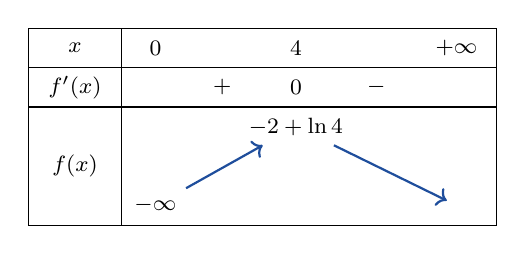
\begin{tikzpicture}[x=0.85cm,y=0.5cm,font=\footnotesize]
\draw (0,0) rectangle (7,-5); \draw (0,-1)--(7,-1); \draw (0,-2)--(7,-2); \draw (1.4,0)--(1.4,-5);
\node at (0.7,-0.5){$x$}; \node at (0.7,-1.5){$f^{\prime}(x)$}; \node at (0.7,-3.5){$f(x)$};
\node at (1.9,-0.5){$0$}; \node at (4,-0.5){$4$}; \node at (6.4,-0.5){$+\infty$};
\node at (2.9,-1.5){$+$}; \node at (4,-1.5){$0$}; \node at (5.2,-1.5){$-$};
\node (a) at (1.9,-4.5){$-\infty$}; \node (b) at (4,-2.5){$-2+\ln4$}; \node (c) at (6.4,-4.5){$$};
\draw[->,cDef,thick] (a)--(b); \draw[->,cDef,thick] (b)--(c);
\end{tikzpicture}\end{LTR}\par (3) لدينا $-2+\ln4\simeq-0{,}61<0$ ، وبالتالي $f(x)\in]-\infty;-2+\ln4]$ أي $f(x)<0$ ، هذا معناه $\ln x-\sqrt x<0$.\par (4) من أجل $x>1$: $0<\ln x<\sqrt x$ ، وبالقسمة على $x>0$: $0<\dfrac{\ln x}x<\dfrac{\sqrt x}x=\dfrac1{\sqrt x}$ ، وبما أن $\lim\limits_{x\to +\infty}\dfrac1{\sqrt x}=0$ فحسب النهاية بالمقارنة: $\lim\limits_{x\to +\infty}\dfrac{\ln x}x=0$.}{35 د}{النشاط يقود إلى النهاية الشهيرة.}
\Row{بناء المعارف}{%
\Lab{cThm}{النهايات الشهيرة}\par\ck\ $\lim\limits_{x\to +\infty}\dfrac{\ln(x)}x=0$.\par
\ck\ $\lim\limits_{\substack{x\to0\\x>0}}x\ln(x)=0$.\par
\Lab{cMeth}{البرهان}\ الأولى من النشاط. الثانية: بوضع $X=\dfrac1x$: $\lim\limits_{\substack{x\to0\\x>0}}x\ln x=\lim\limits_{X\to+\infty}\dfrac1X\ln\left(\dfrac1X\right)=\lim\limits_{X\to+\infty}\left(-\dfrac{\ln X}X\right)=0$.\par}{50 د}{إخراج العامل المشترك.}
\Row{}{%
\Lab{cRem}{ملاحظات}\ التفسير: عند $+\infty$ الدالة $x\mapsto x$ «تتفوق» على الدالة $\ln$.\par\Lab{cEx}{مثال 1}\ $\lim\limits_{x\to +\infty}(x-\ln x)=\lim\limits_{x\to +\infty}x\left(1-\dfrac{\ln x}x\right)=+\infty$.\par}{}{}
\Row{}{%
\Lab{cEx}{مثال 2}\ $\lim\limits_{x\to +\infty}\dfrac{\ln x}{x^2}=\lim\limits_{x\to +\infty}\dfrac{\ln x}x\times\dfrac1x=0$ ؛ $\lim\limits_{x\to +\infty}\dfrac{2\ln x+1}x=\lim\limits_{x\to +\infty}\left(2\dfrac{\ln x}x+\dfrac1x\right)=0$.\par\Lab{cEx}{مثال 3}\ $\lim\limits_{\substack{x\to0\\x>0}}\left(x\ln x-3x+1\right)=1$ ؛ $\lim\limits_{\substack{x\to0\\x>0}}x^2\ln x=\lim\limits_{\substack{x\to0\\x>0}}x\times x\ln x=0$.\par}{}{}
\Row{}{%
\Lab{cThm!80!black}{حذار}\ الشكل $\infty-\infty$ أو $0\times\infty$: نُخرج العامل المشترك لنظهر نهاية شهيرة.}{}{}
\Row{التقويم}{%
\Lab{cMeth}{تمرين تطبيقي}\par $f$ الدالة المعرفة على $]0;+\infty[$ بـ: $f(x)=x-\ln x$.\par (1) احسب $\lim\limits_{x\to 0^{+}}f(x)$ و $\lim\limits_{x\to +\infty}f(x)$. (2) ادرس اتجاه تغير $f$ وشكّل جدول تغيراتها. (3) استنتج أن من أجل كل $x>0$: $\ln x<x$.\par}{25 د}{تقويم فردي.}
\Row{}{%
\Lab{cEx}{حل التمرين التطبيقي}\par (1) $\lim\limits_{x\to 0^{+}}f(x)=+\infty$ (لأن $-\ln x\to+\infty$) ؛ $\lim\limits_{x\to +\infty}f(x)=\lim\limits_{x\to +\infty}x\left(1-\dfrac{\ln x}x\right)=+\infty$.\par (2) $f^{\prime}(x)=1-\dfrac1x=\dfrac{x-1}x$:\par\smallskip\begin{LTR}\centering 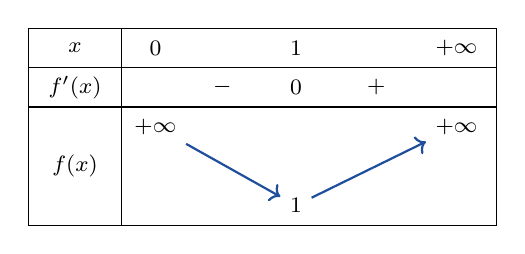
\begin{tikzpicture}[x=0.85cm,y=0.5cm,font=\footnotesize]
\draw (0,0) rectangle (7,-5); \draw (0,-1)--(7,-1); \draw (0,-2)--(7,-2); \draw (1.4,0)--(1.4,-5);
\node at (0.7,-0.5){$x$}; \node at (0.7,-1.5){$f^{\prime}(x)$}; \node at (0.7,-3.5){$f(x)$};
\node at (1.9,-0.5){$0$}; \node at (4,-0.5){$1$}; \node at (6.4,-0.5){$+\infty$};
\node at (2.9,-1.5){$-$}; \node at (4,-1.5){$0$}; \node at (5.2,-1.5){$+$};
\node (a) at (1.9,-2.5){$+\infty$}; \node (b) at (4,-4.5){$1$}; \node (c) at (6.4,-2.5){$+\infty$};
\draw[->,cDef,thick] (a)--(b); \draw[->,cDef,thick] (b)--(c);
\end{tikzpicture}\end{LTR}\par (3) القيمة الحدية الصغرى $f(1)=1>0$ ، إذن $x-\ln x>0$ أي $\ln x<x$.\par\textbf{واجب منزلي:} تمارين من صفحة 143 إلى 147.\par\smallskip\textbf{ملاحظات حول سير الحصة:} \dotfill}{}{}
\end{Sayr}
\newpage
\ModhHead{33}{3 ت ا}{تحليل}{الدالة اللوغاريتمية}{02 سا}{دراسة دوال من الشكل $\ln u$ ، اللوغاريتم العشري}%
{\begin{itemize}\item دراسة $\ln$ ، مشتقة دالة مركبة.\end{itemize}}%
{\begin{itemize}\item دراسة دوال من الشكل $\ln u$.\item الدالة اللوغاريتمية ذات الأساس $a$ ، اللوغاريتم العشري ، أمثلة من المجال الاقتصادي.\end{itemize}}%
{المنهاج ، الكتاب المدرسي ، الآلة الحاسبة ، برمجية Geogebra.}
\begin{Sayr}
\Row{مرحلة الانطلاق}{%
\textbf{التهيئة النفسية:} ما مجموعة تعريف $\ln(2x-4)$ ؟ وكم رقماً يكتب به العدد $2^{100}$ ؟}{10 د}{سؤال.}
\Row{التشخيص والاكتشاف}{%
\Lab{cEx}{نشاط رقم 06}\par\ck\ $\ln u$ معرفة حيث $u(x)>0$ ؛ بمشتقة الدالة المركبة: $\big(\ln u\big)^{\prime}=u^{\prime}\times\dfrac1u$.\par
\ck\ العدد ذو $k$ رقماً يحقق $10^{k-1}\leqslant N<10^k$: نحتاج دالة تحوّل $10^k$ إلى $k$ ، هي $\dfrac{\ln x}{\ln10}$.\par
}{35 د}{مشتقة المركب.}
\Row{بناء المعارف}{%
\Lab{cThm}{الدالة $\ln u$}\par\ck\ $\big(\ln u\big)^{\prime}=\dfrac{u^{\prime}}u$: للدالة $\ln u$ نفس اتجاه تغير $u$.\par
\ck\ دالة أصلية لـ $\dfrac{u^{\prime}}u$ (مع $u>0$) هي $\ln u$.\par
\ck\ النهايات بنهاية دالة مركبة.\par
\Lab{cEx}{مثال}\ $f(x)=\ln(x^2+1)$ على $\mathbb R$: $f^{\prime}(x)=\dfrac{2x}{x^2+1}$ ؛ $\lim\limits_{x\to \pm\infty}f(x)=+\infty$.\par\smallskip\begin{LTR}\centering 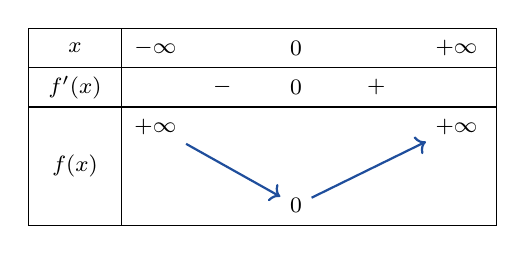
\begin{tikzpicture}[x=0.85cm,y=0.5cm,font=\footnotesize]
\draw (0,0) rectangle (7,-5); \draw (0,-1)--(7,-1); \draw (0,-2)--(7,-2); \draw (1.4,0)--(1.4,-5);
\node at (0.7,-0.5){$x$}; \node at (0.7,-1.5){$f^{\prime}(x)$}; \node at (0.7,-3.5){$f(x)$};
\node at (1.9,-0.5){$-\infty$}; \node at (4,-0.5){$0$}; \node at (6.4,-0.5){$+\infty$};
\node at (2.9,-1.5){$-$}; \node at (4,-1.5){$0$}; \node at (5.2,-1.5){$+$};
\node (a) at (1.9,-2.5){$+\infty$}; \node (b) at (4,-4.5){$0$}; \node (c) at (6.4,-2.5){$+\infty$};
\draw[->,cDef,thick] (a)--(b); \draw[->,cDef,thick] (b)--(c);
\end{tikzpicture}\end{LTR}\par و $\displaystyle\int_0^1\dfrac{2x}{x^2+1}\,dx=\big[\ln(x^2+1)\big]_0^1=\ln2$.\par}{50 د}{الآلة الحاسبة: \fbox{log} و \fbox{ln}.}
\Row{}{%
\Lab{cDef}{اللوغاريتم ذو الأساس $a$}\ من أجل $a>0$ و $a\neq1$: $\log_a x=\dfrac{\ln x}{\ln a}$ ؛ \textbf{اللوغاريتم العشري}: $\log x=\dfrac{\ln x}{\ln10}$ ، و $\log10^n=n$.\par\Lab{cEx}{مثال}\par\ck\ $\log2^{100}=100\log2\simeq30{,}1$: $10^{30}\leqslant2^{100}<10^{31}$ ، إذن $2^{100}$ يكتب بـ $31$ رقماً.\par
\ck\ المقاييس اللوغاريتمية: شدة الصوت بالديسيبل $L=10\log\dfrac I{I_0}$.\par
\ck\ رأس مال بفائدة مركبة $5\%$ يتضاعف لما $1{,}05^n\geqslant2$: $n\geqslant\dfrac{\ln2}{\ln1{,}05}\simeq14{,}2$: بعد $15$ سنة.\par
}{}{}
\Row{التقويم}{%
\Lab{cMeth}{تمرين تطبيقي}\par $g(x)=\ln(2x-4)$. (1) عيّن مجموعة التعريف. (2) احسب النهايات عند طرفيها. (3) ادرس اتجاه تغير $g$. (4) حل $g(x)=0$. (5) كم رقماً للعدد $3^{50}$ ؟\par}{25 د}{نهاية المحور: فرض أو معالجة.}
\Row{}{%
\Lab{cEx}{حل التمرين التطبيقي}\par (1) $2x-4>0$: $D=]2;+\infty[$. (2) $\lim\limits_{x\to 2^{+}}g(x)=-\infty$ ، $\lim\limits_{x\to +\infty}g(x)=+\infty$. (3) $g^{\prime}(x)=\dfrac2{2x-4}=\dfrac1{x-2}>0$: متزايدة تماماً. (4) $2x-4=1$: $x=\dfrac52$. (5) $50\log3\simeq23{,}86$: $24$ رقماً.\par\textbf{واجب منزلي:} تمارين من صفحة 143 إلى 147.\par\smallskip\textbf{ملاحظات حول سير الحصة:} \dotfill}{}{}
\end{Sayr}
\end{document}
